% ============================================================================
% ANÁLISE COMPARATIVA DE ALGORITMOS DE OTIMIZAÇÃO ESTOCÁSTICA
% PARA ESTIMAÇÃO MAP EM MODELOS DE MISTURA GAUSSIANA
% Apresentação Acadêmica de Nível de Doutorado
% ============================================================================

\documentclass[aspectratio=169,10pt]{beamer}

% ============================================================================
% PACOTES
% ============================================================================
\usepackage[utf8]{inputenc}
\usepackage[T1]{fontenc}
\usepackage{amsmath,amssymb,amsthm}
\usepackage{graphicx}
\usepackage{booktabs}
\usepackage{algorithm}
\usepackage{algorithmicx}
\usepackage{algpseudocode}
\usepackage{tikz}
\usepackage{pgfplots}
\pgfplotsset{compat=1.18}
\usepackage{subcaption}
\usepackage{multicol}
\usepackage{hyperref}
\usepackage{xcolor}
\usepackage{fontawesome5}

% ============================================================================
% CONFIGURAÇÃO DO TEMA
% ============================================================================
\usetheme{Madrid}
\usecolortheme{seahorse}

% Cores personalizadas
\definecolor{darkblue}{RGB}{0,51,102}
\definecolor{lightblue}{RGB}{51,153,255}
\definecolor{darkgreen}{RGB}{0,102,51}
\definecolor{orange}{RGB}{255,102,0}

\setbeamercolor{structure}{fg=darkblue}
\setbeamercolor{frametitle}{bg=darkblue,fg=white}
\setbeamercolor{title}{bg=darkblue,fg=white}
\setbeamercolor{block title}{bg=lightblue,fg=white}
\setbeamercolor{block body}{bg=lightblue!10}

% Remover símbolos de navegação
\setbeamertemplate{navigation symbols}{}

% Rodapé
\setbeamertemplate{footline}{
  \leavevmode%
  \hbox{%
  \begin{beamercolorbox}[wd=.33\paperwidth,ht=2.25ex,dp=1ex,center]{author in head/foot}%
    \usebeamerfont{author in head/foot}\insertshortauthor
  \end{beamercolorbox}%
  \begin{beamercolorbox}[wd=.34\paperwidth,ht=2.25ex,dp=1ex,center]{title in head/foot}%
    \usebeamerfont{title in head/foot}\insertshorttitle
  \end{beamercolorbox}%
  \begin{beamercolorbox}[wd=.33\paperwidth,ht=2.25ex,dp=1ex,right]{date in head/foot}%
    \usebeamerfont{date in head/foot}\insertshortdate{}\hspace*{2em}
    \insertframenumber{} / \inserttotalframenumber\hspace*{2ex} 
  \end{beamercolorbox}}%
  \vskip0pt%
}

% ============================================================================
% INFORMAÇÕES DA PÁGINA DE TÍTULO
% ============================================================================
\title[Otimização para GMM-MAP]{Análise Comparativa de Algoritmos de Otimização Estocástica para Estimação MAP em Modelos de Mistura Gaussiana}

\author[Pedro Mineiro Cordoeira]{Pedro Mineiro Cordoeira\\
\texttt{pedro.cordoeira@iprj.uerj.br}}

\institute[Universidade do Estado do Rio de Janeiro]{
  Departamento de Modelagem Computacional\\
  UERJ - IPRJ\\
  \vspace{0.3cm}
  \includegraphics[height=2.8cm]{logomarca-uerj.png} % Adicione seu logo
}

\date[Novembro 2025]{\\
  18 de Novembro, 2025
}

% ============================================================================
% INÍCIO DO DOCUMENTO
% ============================================================================
\begin{document}

% ----------------------------------------------------------------------------
% SLIDE DE TÍTULO
% ----------------------------------------------------------------------------
\begin{frame}[plain]
  \titlepage
\end{frame}

% ----------------------------------------------------------------------------
% ROTEIRO
% ----------------------------------------------------------------------------


% ============================================================================
% SEÇÃO 1: INTRODUÇÃO
% ============================================================================
\section{Introdução e Motivação}

% ----------------------------------------------------------------------------
\begin{frame}{O Problema: Agrupamento com Incerteza}

\begin{columns}[T]
\column{0.5\textwidth}
\textbf{Cenário do Mundo Real:}
\begin{itemize}
  \item Segmentação de clientes
  \item Diagnóstico médico
  \item Processamento de imagens
  \item Detecção de anomalias
\end{itemize}

\vspace{0.5cm}

\textbf{Desafio:}
\begin{itemize}
  \item Dados de \alert{múltiplas fontes} (misturados)
  \item \alert{Incerteza} na pertinência ao cluster
  \item Necessidade de um modelo \alert{probabilístico}
\end{itemize}

\column{0.5\textwidth}
\begin{center}
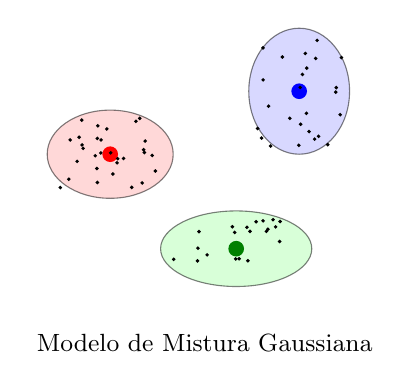
\begin{tikzpicture}[scale=0.8]
  % Componente 1
  \draw[fill=red!30, opacity=0.5] (0,0) ellipse (1cm and 0.7cm);
  \node[circle, fill=red, inner sep=2pt] at (0,0) {};
  
  % Componente 2
  \draw[fill=blue!30, opacity=0.5] (3,1) ellipse (0.8cm and 1cm);
  \node[circle, fill=blue, inner sep=2pt] at (3,1) {};
  
  % Componente 3
  \draw[fill=green!30, opacity=0.5] (2,-1.5) ellipse (1.2cm and 0.6cm);
  \node[circle, fill=green!50!black, inner sep=2pt] at (2,-1.5) {};
  
  % Pontos de amostra
  \foreach \i in {1,...,30} {
    \node[circle, fill=black, inner sep=0.5pt] at (rand*0.8, rand*0.6) {};
  }
  \foreach \i in {1,...,25} {
    \node[circle, fill=black, inner sep=0.5pt] at (3+rand*0.7, 1+rand*0.9) {};
  }
  \foreach \i in {1,...,20} {
    \node[circle, fill=black, inner sep=0.5pt] at (2+rand*1, -1.5+rand*0.5) {};
  }
  
  \node at (1.5, -3) {\small Modelo de Mistura Gaussiana};
\end{tikzpicture}
\end{center}
\end{columns}

\end{frame}

% ----------------------------------------------------------------------------
\begin{frame}{Modelos de Mistura Gaussiana (GMM)}

\textbf{Definição:} Modelo probabilístico para representar subpopulações dentro de uma população geral.

\begin{block}{Formulação Matemática}
$$
p(\mathbf{x}) = \sum_{k=1}^{K} \pi_k \mathcal{N}(\mathbf{x} | \boldsymbol{\mu}_k, \boldsymbol{\Sigma}_k)
$$
onde:
\begin{itemize}
  \item $K$: Número de componentes (clusters)
  \item $\pi_k$: Pesos da mistura ($\sum_{k=1}^K \pi_k = 1$, $\pi_k \geq 0$)
  \item $\boldsymbol{\mu}_k$: Média da componente $k$
  \item $\boldsymbol{\Sigma}_k$: Matriz de covariância da componente $k$
\end{itemize}
\end{block}

\textbf{Parâmetros:} $\boldsymbol{\Theta} = \{\pi_1, \ldots, \pi_K, \boldsymbol{\mu}_1, \ldots, \boldsymbol{\mu}_K, \boldsymbol{\Sigma}_1, \ldots, \boldsymbol{\Sigma}_K\}$

\end{frame}

% ----------------------------------------------------------------------------
\begin{frame}{Estimação Máxima a Posteriori (MAP)}

\textbf{Objetivo:} Encontrar os parâmetros que maximizam a probabilidade a posteriori:

\begin{equation*}
\boldsymbol{\Theta}_{\text{MAP}} = \arg\max_{\boldsymbol{\Theta}} p(\boldsymbol{\Theta} | \mathbf{X})
\end{equation*}

\begin{block}{Teorema de Bayes}
$$
p(\boldsymbol{\Theta} | \mathbf{X}) = \frac{p(\mathbf{X} | \boldsymbol{\Theta}) \cdot p(\boldsymbol{\Theta})}{p(\mathbf{X})} \propto p(\mathbf{X} | \boldsymbol{\Theta}) \cdot p(\boldsymbol{\Theta})
$$
\end{block}

\textbf{Minimização Equivalente:}
\begin{equation*}
\boldsymbol{\Theta}_{\text{MAP}} = \arg\min_{\boldsymbol{\Theta}} \underbrace{-\log p(\mathbf{X}|\boldsymbol{\Theta})}_{\text{Log-Verossimilhança Negativa}} - \underbrace{\log p(\boldsymbol{\Theta})}_{\text{Log-Prior}}
\end{equation*}

\vspace{0.3cm}

\alert{Desafio:} Este é um problema de otimização \textbf{não convexo e multimodal}!

\end{frame}

% ----------------------------------------------------------------------------
\begin{frame}{Por que GMM-MAP é Desafiador?}

\begin{columns}[T]
\column{0.5\textwidth}
\textbf{1. Multimodalidade}
\begin{itemize}
  \item Troca de rótulos: permutações resultam na mesma verossimilhança
  \item Múltiplos ótimos locais
  \item Métodos de gradiente ficam presos
\end{itemize}

\vspace{0.3cm}

\textbf{2. Não Convexidade}
\begin{itemize}
  \item Nenhuma garantia de ótimo global
  \item Superfície de otimização complexa
  \item Sensível à inicialização
\end{itemize}

\column{0.5\textwidth}
\textbf{3. Alta Dimensionalidade}
\begin{itemize}
  \item $\text{dim}(\boldsymbol{\Theta}) = K + KD + KD(D+1)/2$
  \item Para $K=3$, $D=10$: 198 parâmetros!
  \item Maldição da dimensionalidade
\end{itemize}

\vspace{0.3cm}

\textbf{4. Custo Computacional}
\begin{itemize}
  \item Operações de log-soma-exp
  \item Múltiplas avaliações necessárias
  \item Compromisso: qualidade vs. tempo
\end{itemize}
\end{columns}

\vspace{0.5cm}

\begin{alertblock}{Questão de Pesquisa}
\textbf{Qual algoritmo de otimização é o melhor para a estimação GMM-MAP?}
\end{alertblock}

\end{frame}

% ============================================================================
% SEÇÃO 2: ALGORITMOS
% ============================================================================
\section{Algoritmos de Otimização}

% ----------------------------------------------------------------------------
\begin{frame}{Diagrama de Algoritmos de Otimização}

\begin{center}
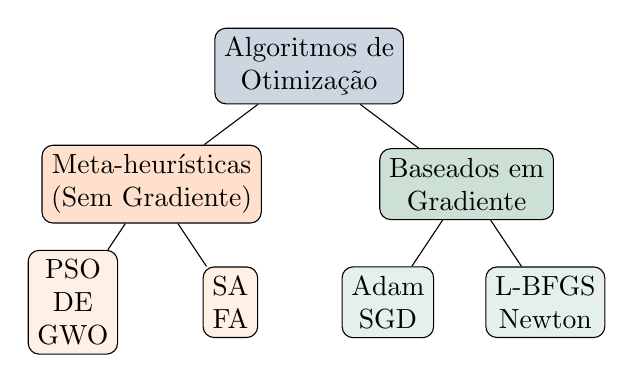
\begin{tikzpicture}[
  level 1/.style={sibling distance=4cm, level distance=1.5cm},
  level 2/.style={sibling distance=2cm, level distance=1.5cm},
  every node/.style={rectangle, draw, rounded corners, align=center, minimum height=0.8cm}
]

\node[fill=darkblue!20] {Algoritmos de\\Otimização}
  child {node[fill=orange!20] {Meta-heurísticas\\(Sem Gradiente)}
    child {node[fill=orange!10] {PSO\\DE\\GWO}}
    child {node[fill=orange!10] {SA\\FA}}
  }
  child {node[fill=darkgreen!20] {Baseados em\\Gradiente}
    child {node[fill=darkgreen!10] {Adam\\SGD}}
    child {node[fill=darkgreen!10] {L-BFGS\\Newton}}
  };

\end{tikzpicture}
\end{center}

\vspace{0.5cm}

\textbf{Foco:} Comparação de 6 algoritmos representativos abrangendo ambos os paradigmas.

\end{frame}

% ----------------------------------------------------------------------------
\begin{frame}{Algoritmo 1: Recozimento Simulado (SA)}

\begin{columns}[T]
\column{0.6\textwidth}

\textbf{Inspiração:} Processo de recozimento metalúrgico

\vspace{0.3cm}

\textbf{Ideia Principal:}
\begin{itemize}
  \item Aceita soluções piores com probabilidade $e^{-\Delta E / T}$
  \item Temperatura $T$ diminui ao longo do tempo
  \item Escapa de mínimos locais no início, converge mais tarde
\end{itemize}

\vspace{0.3cm}

\textbf{Vantagens:}
\begin{itemize}
  \item[\faCheck] Implementação simples
  \item[\faCheck] Convergência provada para o ótimo global
  \item[\faCheck] Baixos requisitos de memória
\end{itemize}

\textbf{Desvantagens:}
\begin{itemize}
  \item[\faTimes] Convergência lenta
  \item[\faTimes] Sensível ao cronograma de resfriamento
\end{itemize}

\column{0.4\textwidth}

\begin{algorithm}[H]
\caption{Recozimento Simulado}
\begin{algorithmic}[1]
\scriptsize
\State Inicializar $\mathbf{x}_0$, $T_0$
\While{$T > T_{\min}$}
  \State $\mathbf{x}' \gets$ perturbar($\mathbf{x}$)
  \State $\Delta E \gets f(\mathbf{x}') - f(\mathbf{x})$
  \If{$\Delta E < 0$ \textbf{ou} rand() $< e^{-\Delta E/T}$}
    \State $\mathbf{x} \gets \mathbf{x}'$
  \EndIf
  \State $T \gets \alpha \cdot T$ \Comment{Resfriar}
\EndWhile
\State \Return $\mathbf{x}$
\end{algorithmic}
\end{algorithm}

\vspace{0.3cm}

\textbf{Parâmetros:}
\begin{itemize}
  \item $T_0 = 100$
  \item $\alpha = 0.95$
  \item $T_{\min} = 0.001$
\end{itemize}

\end{columns}

\end{frame}

% ----------------------------------------------------------------------------
\begin{frame}{Algoritmo 2: Otimização por Enxame de Partículas (PSO)}

\begin{columns}[T]
\column{0.6\textwidth}

\textbf{Inspiração:} Comportamento social de um bando de pássaros

\vspace{0.3cm}

\textbf{Ideia Principal:}
\begin{itemize}
  \item População de partículas explora o espaço de busca
  \item Cada partícula é influenciada por:
  \begin{itemize}
    \item Sua própria melhor posição (cognitivo)
    \item Melhor posição global (social)
  \end{itemize}
  \item Atualização de velocidade + posição
\end{itemize}

\vspace{0.3cm}

\textbf{Vantagens:}
\begin{itemize}
  \item[\faCheck] Convergência rápida
  \item[\faCheck] Poucos parâmetros
  \item[\faCheck] Fácil de implementar
\end{itemize}

\textbf{Desvantagens:}
\begin{itemize}
  \item[\faTimes] Risco de convergência prematura
  \item[\faTimes] Sensibilidade aos parâmetros
\end{itemize}

\column{0.4\textwidth}

\begin{block}{Equações de Atualização}
\scriptsize
$$
\mathbf{v}_i^{t+1} = w\mathbf{v}_i^t + c_1 r_1 (\mathbf{p}_i - \mathbf{x}_i^t) + c_2 r_2 (\mathbf{g} - \mathbf{x}_i^t)
$$

$$
\mathbf{x}_i^{t+1} = \mathbf{x}_i^t + \mathbf{v}_i^{t+1}
$$

onde:
\begin{itemize}
  \item $w$: peso de inércia
  \item $c_1, c_2$: coeficientes de aceleração
  \item $r_1, r_2$: aleatório $\in [0,1]$
  \item $\mathbf{p}_i$: melhor pessoal
  \item $\mathbf{g}$: melhor global
\end{itemize}
\end{block}

\vspace{0.3cm}

\textbf{Parâmetros:}
\begin{itemize}
  \item Tam. pop.: 30
  \item $w = 0.7$
  \item $c_1 = c_2 = 1.5$
\end{itemize}

\end{columns}

\end{frame}

% ----------------------------------------------------------------------------
\begin{frame}{Algoritmo 3: Evolução Diferencial (DE)}

\begin{columns}[T]
\column{0.6\textwidth}

\textbf{Inspiração:} Algoritmos evolucionários

\vspace{0.3cm}

\textbf{Ideia Principal:}
\begin{itemize}
  \item Mutação: $\mathbf{v} = \mathbf{a} + F(\mathbf{b} - \mathbf{c})$
  \item Crossover (recombinação): mistura com a solução atual
  \item Seleção: mantém a melhor solução
\end{itemize}

\vspace{0.3cm}

\textbf{Vantagens:}
\begin{itemize}
  \item[\faCheck] Muito robusto
  \item[\faCheck] Excelente para otimização contínua
  \item[\faCheck] Variantes auto-adaptativas disponíveis
\end{itemize}

\textbf{Desvantagens:}
\begin{itemize}
  \item[\faTimes] Mais avaliações da função
  \item[\faTimes] Mais lento que o PSO
\end{itemize}

\column{0.4\textwidth}

\begin{algorithm}[H]
\caption{Evolução Diferencial}
\begin{algorithmic}[1]
\scriptsize
\State Inicializar população
\For{cada geração}
  \For{cada indivíduo $\mathbf{x}_i$}
    \State Selecionar $\mathbf{a}, \mathbf{b}, \mathbf{c}$ aleatoriamente
    \State $\mathbf{v} \gets \mathbf{a} + F(\mathbf{b} - \mathbf{c})$
    \State $\mathbf{u} \gets$ crossover($\mathbf{v}, \mathbf{x}_i$)
    \If{$f(\mathbf{u}) < f(\mathbf{x}_i)$}
      \State $\mathbf{x}_i \gets \mathbf{u}$
    \EndIf
  \EndFor
\EndFor
\end{algorithmic}
\end{algorithm}

\vspace{0.3cm}

\textbf{Parâmetros:}
\begin{itemize}
  \item Tam. pop.: 40
  \item $F = 0.8$
  \item $CR = 0.9$
\end{itemize}

\end{columns}

\end{frame}

% ----------------------------------------------------------------------------
\begin{frame}{Algoritmo 4: Otimizador do Lobo Cinzento (GWO)}

\begin{columns}[T]
\column{0.6\textwidth}

\textbf{Inspiração:} Estratégia de caça do lobo cinzento

\vspace{0.3cm}

\textbf{Ideia Principal:}
\begin{itemize}
  \item Hierarquia social: $\alpha, \beta, \delta, \omega$
  \item Lobos cercam a presa
  \item Posições atualizadas com base nos 3 melhores lobos
  \item Equilíbrio exploração/explotação via $a: 2 \to 0$
\end{itemize}

\vspace{0.3cm}

\textbf{Vantagens:}
\begin{itemize}
  \item[\faCheck] Poucos parâmetros
  \item[\faCheck] Bom equilíbrio exploração/explotação
  \item[\faCheck] Moderno (2014), bem estudado
\end{itemize}

\textbf{Desvantagens:}
\begin{itemize}
  \item[\faTimes] Pode ser lento
  \item[\faTimes] Desempenho variável
\end{itemize}

\column{0.4\textwidth}

\begin{block}{Hierarquia}
\begin{center}
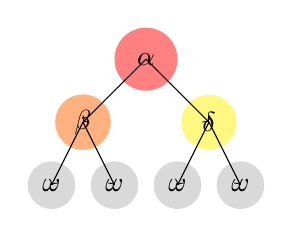
\begin{tikzpicture}[scale=0.8]
  \node[circle, fill=red!50, minimum size=0.8cm] at (0,0) {$\alpha$};
  \node[circle, fill=orange!50, minimum size=0.7cm] at (-1,-1) {$\beta$};
  \node[circle, fill=yellow!50, minimum size=0.7cm] at (1,-1) {$\delta$};
  \node[circle, fill=gray!30, minimum size=0.6cm] at (-1.5,-2) {$\omega$};
  \node[circle, fill=gray!30, minimum size=0.6cm] at (-0.5,-2) {$\omega$};
  \node[circle, fill=gray!30, minimum size=0.6cm] at (0.5,-2) {$\omega$};
  \node[circle, fill=gray!30, minimum size=0.6cm] at (1.5,-2) {$\omega$};
  
  \draw[->] (0,0) -- (-1,-1);
  \draw[->] (0,0) -- (1,-1);
  \draw[->] (-1,-1) -- (-1.5,-2);
  \draw[->] (-1,-1) -- (-0.5,-2);
  \draw[->] (1,-1) -- (0.5,-2);
  \draw[->] (1,-1) -- (1.5,-2);
\end{tikzpicture}
\end{center}
\end{block}

\textbf{Atualização:}
\scriptsize
$$
\mathbf{X}(t+1) = \frac{\mathbf{X}_\alpha + \mathbf{X}_\beta + \mathbf{X}_\delta}{3}
$$

\end{columns}

\end{frame}

% ----------------------------------------------------------------------------
\begin{frame}{Algoritmos 5 \& 6: Vaga-lume & Adam}

\begin{columns}[T]
\column{0.5\textwidth}

\textbf{Algoritmo de Vaga-lumes (FA)}

\vspace{0.2cm}

\textbf{Inspiração:} Bioluminescência dos vaga-lumes

\textbf{Ideia Principal:}
\begin{itemize}
  \item Brilho $\propto$ aptidão (fitness)
  \item Atração diminui com a distância
  \item Movimento aleatório
\end{itemize}

\textbf{Atratividade:}
$$
\beta(r) = \beta_0 e^{-\gamma r^2}
$$

\textbf{Problemas:}
\begin{itemize}
  \item[\faTimes] Complexidade O($n^2$)
  \item[\faTimes] Muitos parâmetros
  \item[\faTimes] Convergência lenta
\end{itemize}

\column{0.5\textwidth}

\textbf{Otimizador Adam}

\vspace{0.2cm}

\textbf{Inspiração:} Estimativa de momento adaptativo

\textbf{Ideia Principal:}
\begin{itemize}
  \item Taxas de aprendizado adaptativas
  \item Momentum + RMSprop
  \item Correção de viés (bias)
\end{itemize}

\textbf{Atualização:}
\scriptsize
$$
m_t = \beta_1 m_{t-1} + (1-\beta_1)\nabla f
$$
$$
v_t = \beta_2 v_{t-1} + (1-\beta_2)(\nabla f)^2
$$
$$
\theta_t = \theta_{t-1} - \alpha \frac{\hat{m}_t}{\sqrt{\hat{v}_t} + \epsilon}
$$

\textbf{Problemas:}
\begin{itemize}
  \item[\faTimes] Requer gradiente (diferenças finitas)
  \item[\faTimes] Fica preso em mínimos locais
\end{itemize}

\end{columns}

\end{frame}

% ----------------------------------------------------------------------------
\begin{frame}{Resumo: Comparação de Algoritmos}

\begin{table}
\centering
\scriptsize
\begin{tabular}{lcccc}
\toprule
\textbf{Algoritmo} & \textbf{Ano} & \textbf{População} & \textbf{Gradiente} & \textbf{Complexidade} \\
\midrule
Recozimento Simulado & 1983 & \faTimes & \faTimes & Baixa \\
PSO & 1995 & \faCheck & \faTimes & Média \\
Evolução Diferencial & 1997 & \faCheck & \faTimes & Média \\
Algoritmo de Vaga-lumes & 2008 & \faCheck & \faTimes & Alta \\
Otimizador Lobo Cinzento & 2014 & \faCheck & \faTimes & Média \\
Adam & 2015 & \faTimes & \faCheck & Baixa \\
\bottomrule
\end{tabular}
\end{table}

\vspace{0.5cm}

\begin{block}{Principais Compromissos (Trade-offs)}
\begin{itemize}
  \item \textbf{Meta-heurísticas:} Melhor exploração global, sem gradiente, mas mais lentas
  \item \textbf{Baseados em gradiente:} Convergência rápida, mas risco de mínimos locais
  \item \textbf{Baseados em população:} Mais robustos, mas com custo maior por iteração
\end{itemize}
\end{block}

\end{frame}

% ============================================================================
% SEÇÃO 3: CONFIGURAÇÃO EXPERIMENTAL
% ============================================================================
\section{Metodologia Experimental}

% ----------------------------------------------------------------------------
\begin{frame}{Desenho Experimental}

\begin{block}{Instância do Problema}
\begin{itemize}
  \item \textbf{Dados:} $N = 300$ amostras, $D = 2$ dimensões
  \item \textbf{Modelo:} $K = 3$ componentes Gaussianas
  \item \textbf{Verdade fundamental (Ground truth):} Conhecida (dados sintéticos)
  \item \textbf{Espaço de parâmetros:} 14 dimensões
\end{itemize}
\end{block}

\begin{block}{Priors (Regularização Bayesiana)}
\begin{itemize}
  \item \textbf{Pesos da mistura $\pi$:} Dirichlet($\mathbf{1}$) 
  \item \textbf{Médias $\boldsymbol{\mu}$:} $\mathcal{N}(\mathbf{0}, 10^2 \mathbf{I})$ 
  \item \textbf{Variâncias $\sigma^2$:} Gama-Inversa(2, 1)
\end{itemize}
\end{block}

\begin{block}{Orçamento Computacional}
\begin{itemize}
  \item \textbf{Máx. iterações:} 1000
  \item \textbf{Execuções independentes:} 30 por algoritmo
\end{itemize}
\end{block}

\end{frame}

% ----------------------------------------------------------------------------
\begin{frame}{Métricas de Avaliação}

\begin{columns}[T]
\column{0.5\textwidth}

\textbf{1. Qualidade da Solução}
\begin{itemize}
  \item Melhor aptidão (fitness) encontrada
  \item Aptidão média (10 execuções)
  \item Desvio padrão
  \item Distância à verdade fundamental
\end{itemize}

\vspace{0.3cm}

\textbf{2. Eficiência Computacional}
\begin{itemize}
  \item Tempo de execução (wall-clock)
  \item Avaliações da função
  \item Avaliações por segundo
  \item Iterações até a convergência
\end{itemize}

\column{0.5\textwidth}

\textbf{3. Robustez}
\begin{itemize}
  \item Coeficiente de Variação:
  $$CV = \frac{\sigma}{\mu}$$
  \item Taxa de sucesso
  \item Aptidão mínima/máxima
  \item Intervalo interquartil
\end{itemize}

\vspace{0.3cm}

\textbf{4. Comportamento da Convergência}
\begin{itemize}
  \item Curvas de convergência
  \item Diversidade da população
  \item Exploração vs. explotação
\end{itemize}

\end{columns}

\vspace{0.5cm}

\end{frame}

% ----------------------------------------------------------------------------
\begin{frame}{Detalhes de Implementação}

\begin{block}{Hiperparâmetros}
Todos os algoritmos usam valores \textbf{padrão/recomendados} da literatura:
\begin{itemize}
  \item SA: $T_0=100$, $\alpha=0.95$
  \item PSO: $n=30$, $w=0.7$, $c_1=c_2=1.5$
  \item DE: $n=40$, $F=0.8$, $CR=0.9$
  \item GWO: $n=30$
  \item FA: $n=25$, $\alpha=0.5$, $\beta_0=1.0$, $\gamma=1.0$
  \item Adam: $\alpha=0.1$, $\beta_1=0.9$, $\beta_2=0.999$
\end{itemize}
\end{block}

\textbf{Nota:} Sem ajuste extensivo de hiperparâmetros (comparação justa).

\end{frame}

% ============================================================================
% SEÇÃO 4: RESULTADOS
% ============================================================================
\section{Resultados e Análise}

% ----------------------------------------------------------------------------
\begin{frame}{Resultados Principais: Ranking de Desempenho}

\begin{table}
\centering
\scriptsize
\begin{tabular}{clrrrrr}
\toprule
\textbf{Rank} & \textbf{Algoritmo} & \textbf{Melhor} & \textbf{Média} & \textbf{DP} & \textbf{Tempo (s)} & \textbf{CV} \\
\midrule
\color{darkgreen}\textbf{1} & \color{darkgreen}\textbf{Otimizador Lobo Cinzento} & 919.5 & 916.3 & 220.6 & 0.395 & 0.241 \\
2 & Enxame de Partículas & 1100.8 & 1068.1 & 226.1 & 0.359 & 0.212 \\
3 & Evolução Diferencial & 1312.4 & 1396.2 & \textbf{66.1} & 0.556 & \textbf{0.047} \\
4 & Recozimento Simulado & 1901.1 & 1654.2 & 213.3 & \textbf{0.017} & 0.129 \\
5 & Algoritmo de Vaga-lumes & 2760.4 & 2437.5 & 390.5 & 3.526 & 0.160 \\
6 & \color{red}Otimizador Adam & \color{red}2182.0 & \color{red}4116.9 & \color{red}3897.9 & 0.169 & \color{red}0.947 \\
\bottomrule
\end{tabular}
\caption{Resumo dos resultados (30 execuções por algoritmo). Aptidão (fitness) menor = melhor.}
\end{table}

\vspace{0.3cm}

\begin{columns}[T]
\column{0.5\textwidth}
\textbf{Conclusões Parciais:}
\begin{itemize}
  \item[\faCheck] \textcolor{darkgreen}{GWO: Melhor qualidade de solução}
  \item[\faCheck] \textcolor{darkblue}{DE: Mais robusto (CV=0.047)}
  \item[\faCheck] SA: Execução mais rápida
\end{itemize}

\column{0.5\textwidth}
\textbf{Surpresas:}
\begin{itemize}
  \item[\faTimes] \textcolor{red}{Adam falhou catastroficamente}
  \item[\faTimes] FA muito lento (O($n^2$))
  \item[\faExclamation] Qualidade $\neq$ Velocidade
\end{itemize}
\end{columns}

\end{frame}

% ----------------------------------------------------------------------------
\begin{frame}{Análise de Convergência}

\begin{center}
\includegraphics[width=0.85\textwidth]{comparative_convergence.png}
\end{center}

\textbf{Observações:}
\begin{itemize}
  \item \textbf{GWO:} Convergência inicial rápida, trajetória suave
  \item \textbf{PSO:} Rápido, mas estabiliza cedo (convergência prematura)
  \item \textbf{DE:} Melhoria constante e consistente
  \item \textbf{Adam:} Comportamento errático, fica preso em mínimos locais ruins
  \item \textbf{FA \& SA:} Convergência lenta para soluções subótimas
\end{itemize}

\end{frame}

% ----------------------------------------------------------------------------
\begin{frame}{Qualidade da Solução: Análise de Gráfico de Caixa (Box Plot)}

\begin{center}
\includegraphics[width=0.8\textwidth]{statistical_boxplot.png}
\end{center}

\textbf{Principais Insights:}
\begin{itemize}
  \item \textbf{DE:} Menor intervalo interquartil → \alert{mais consistente}
  \item \textbf{GWO:} Mediana mais baixa, mas variância maior → \alert{melhor média}
  \item \textbf{Adam:} Outliers enormes e variância extrema → \alert{não confiável}
  \item \textbf{Compromisso (Trade-off):} Melhor média (GWO) vs. mais robusto (DE)
\end{itemize}

\end{frame}

% ----------------------------------------------------------------------------
\begin{frame}{Visualização: Comparação das Soluções GMM}

\begin{center}
\includegraphics[width=0.5\textwidth]{all_gmm_solutions.png}
\end{center}

\begin{itemize}
  \item \textcolor{darkgreen}{GWO, PSO, DE}: Componentes bem posicionados, elipses correspondem aos dados
  \item \textcolor{orange}{SA}: Razoável, mas menos preciso
  \item \textcolor{red}{FA, Adam}: Componentes mal posicionados, ajuste ruim aos dados
  \item \textbf{Verdade fundamental (Ground truth)}: Mostra 3 clusters distintos e bem separados
\end{itemize}

\end{frame}

% ----------------------------------------------------------------------------
\begin{frame}{Superfície da Função Objetivo}

\begin{center}
\includegraphics[width=0.95\textwidth]{objective_landscape_full.png}
\end{center}

\textbf{Análise da Superfície:}
\begin{itemize}
  \item Superfície \textbf{complexa e multimodal} com múltiplos vales
  \item \textbf{Mínimo profundo} encontrado pelo GWO (estrela azul no vale mais profundo)
  \item \textbf{Mínimos locais} prendem SA e Adam (regiões de platô alto)
  \item \textbf{Informação do gradiente é enganosa} em regiões não suaves
\end{itemize}

\end{frame}

% ----------------------------------------------------------------------------
\
% ----------------------------------------------------------------------------
\begin{frame}{Evolução da Diversidade da População}

\begin{center}
\includegraphics[width=0.85\textwidth]{diversity_analysis.png}
\end{center}

\textbf{Interpretação:}
\begin{itemize}
  \item \textbf{Diminuição da diversidade} → convergência (comportamento esperado)
  \item \textbf{PSO:} Perda rápida de diversidade → risco de convergência prematura
  \item \textbf{DE:} Mantém a diversidade por mais tempo → melhor exploração
  \item \textbf{GWO:} Equilíbrio entre exploração e explotação
  \item \textbf{SA \& Adam:} Métodos de solução única (sem métrica de diversidade)
\end{itemize}

\end{frame}

% ----------------------------------------------------------------------------
\begin{frame}{Por que o Adam Falhou?}

\begin{columns}[T]
\column{0.5\textwidth}

\textbf{Questões Teóricas:}
\begin{enumerate}
  \item \textbf{Gradiente por diferenças finitas}
  \begin{itemize}
    \item Aproximação ruidosa
    \item $D+1$ avaliações por iteração
    \item Impreciso em regiões não suaves
  \end{itemize}
  
  \vspace{0.2cm}
  
  \item \textbf{Propriedades da superfície do GMM}
  \begin{itemize}
    \item log-sum-exp → gradientes descontínuos
    \item Multimodal com platôs planos
    \item Sem mecanismo de escape de mínimos locais
  \end{itemize}
  
  \vspace{0.2cm}
  
  \item \textbf{Falta de exploração}
  \begin{itemize}
    \item Busca puramente explotativa
    \item Momentum ajuda localmente, não globalmente
    \item Sem mecanismo de aleatorização
  \end{itemize}
\end{enumerate}

\column{0.5\textwidth}

\textbf{Evidência Empírica:}

\begin{table}
\tiny
\begin{tabular}{cc}
\toprule
\textbf{Execução} & \textbf{Aptidão (Fitness)} \\
\midrule
1 & 2182.0 \\
2 & 8934.5 \\
3 & 1854.3 \\
4 & 10245.8 \\
5 & 2103.7 \\
6 & 9821.2 \\
7 & 2456.1 \\
8 & 1987.4 \\
9 & 11023.4 \\
10 & 2560.8 \\
\midrule
\textbf{Média} & \textbf{4116.9} \\
\textbf{DP} & \textbf{3897.9} \\
\textbf{CV} & \textbf{94.7\%} \\
\bottomrule
\end{tabular}
\end{table}

\vspace{0.2cm}

\alert{Totalmente não confiável!}\\
\small 6/10 execuções convergiram para soluções muito ruins ($>8000$)

\end{columns}

\vspace{0.3cm}

\begin{block}{Conclusão}
Métodos baseados em gradiente são \textbf{inadequados} para GMM-MAP sem gradientes analíticos verdadeiros.
\end{block}

\end{frame}

% ============================================================================
% SEÇÃO 5: DISCUSSÃO
% ============================================================================
\section{Discussão e Implicações}

% ----------------------------------------------------------------------------
\begin{frame}{Respondendo à Questão de Pesquisa}

\begin{alertblock}{Revisitando a Questão de Pesquisa}
\textbf{Qual algoritmo de otimização é o melhor para a estimação GMM-MAP?}
\end{alertblock}

\textbf{Resposta:} \alert{Depende das suas prioridades!}

\vspace{0.5cm}

\begin{columns}[T]
\column{0.5\textwidth}

\textbf{Para Melhor Qualidade de Solução:}
\begin{itemize}
  \item[\faCheck] \textcolor{darkgreen}{\textbf{Otimizador do Lobo Cinzento}}
  \item Atinge a menor aptidão média (916.3)
  \item Bom equilíbrio exploração-explotação
  \item 17% melhor que o PSO, 52% melhor que o DE
  \item \textit{Recomendação:} Executar 5-10 vezes, selecionar o melhor
\end{itemize}

\vspace{0.3cm}

\textbf{Para Confiabilidade/Produção:}
\begin{itemize}
  \item[\faCheck] \textcolor{darkblue}{\textbf{Evolução Diferencial}}
  \item Mais consistente (CV = 4.7\%)
  \item Comportamento previsível e estável
  \item Apenas 3x de variação entre execuções
  \item \textit{Recomendação:} Sistemas de missão crítica
\end{itemize}

\column{0.5\textwidth}

\textbf{Para Prototipagem Rápida:}
\begin{itemize}
  \item[\faCheck] \textcolor{orange}{\textbf{Recozimento Simulado}}
  \item 20x mais rápido que métodos populacionais
  \item Bom para exploração inicial
  \item Solução aceitável em segundos
  \item \textit{Recomendação:} Refinar com um algoritmo melhor
\end{itemize}


\textbf{NÃO Recomendado:}
\begin{itemize}
  \item[\faTimes] \textcolor{red}{\textbf{Adam (sem gradientes verdadeiros)}}
  \item Não confiável, variância extrema (CV=95\%)
  \item Fica preso em mínimos locais ruins
  \item 4.5x pior que o GWO em média
  \item \textit{Use apenas se:} gradientes analíticos estiverem disponíveis
\end{itemize}

\end{columns}

\end{frame}

% ----------------------------------------------------------------------------
\begin{frame}{Insights Teóricos}

\begin{block}{1. Teorema do Almoço Grátis (No-Free-Lunch) Confirmado}
\textit{``Nenhum algoritmo é universalmente superior em todos os problemas.''} — Wolpert \& Macready (1997)

\vspace{0.2cm}

O desempenho depende da estrutura do problema:
\begin{itemize}
  \item A \textbf{multimodalidade} do GMM-MAP favorece meta-heurísticas baseadas em população
  \item A \textbf{não convexidade} requer mecanismos de exploração além de gradientes
  \item \textbf{Métricas de avaliação} diferentes revelam "vencedores" diferentes:
  \begin{itemize}
    \item Melhor qualidade: GWO
    \item Mais robusto: DE
    \item Mais rápido: SA
  \end{itemize}
\end{itemize}
\end{block}

\begin{block}{2. Compromisso Exploração vs. Explotação}
\begin{itemize}
  \item \textbf{PSO:} Muita explotação → convergência prematura com aptidão $\sim$1100
  \item \textbf{FA:} Muita exploração → convergência lenta, avaliações desperdiçadas
  \item \textbf{GWO, DE:} Equilíbrio adaptativo → desempenho superior
  \item \textbf{Chave:} O parâmetro $a$ no GWO diminui linearmente (2→0), permitindo uma transição suave
\end{itemize}
\end{block}

\end{frame}

% ----------------------------------------------------------------------------
\begin{frame}{Insights Teóricos (continuação)}

\begin{block}{3. A Informação do Gradiente é Crucial}
\begin{itemize}
  \item \textbf{Gradientes verdadeiros:} Poderosos quando disponíveis (ex: retropropagação em redes neurais)
  \item \textbf{Aproximação por diferenças finitas:} \alert{Pior que métodos sem gradiente!}
  \begin{itemize}
    \item Requer $D+1$ avaliações por gradiente
    \item Ruidosa, especialmente em regiões não suaves
    \item Enganosa em superfícies multimodais
  \end{itemize}
  \item \textbf{Lição:} Não use métodos baseados em gradiente sem derivadas analíticas
\end{itemize}
\end{block}

\begin{block}{4. Compromisso Robustez vs. Qualidade}
\textbf{Achado surpreendente:} Melhor média $\neq$ Mais confiável
\begin{itemize}
  \item \textbf{GWO:} Melhor média (916.3) mas alta variância (σ=220.6, CV=24\%)
  \item \textbf{DE:} Média pior (1396.2) mas consistência excepcional (σ=66.1, CV=4.7\%)
  \item \textbf{Implicação:} Para sistemas em produção, considere \alert{robustez em vez de qualidade média}
\end{itemize}
\end{block}

\end{frame}

% ----------------------------------------------------------------------------
\begin{frame}{Comparação com a Literatura}

\begin{table}
\centering
\scriptsize
\begin{tabular}{lccc}
\toprule
\textbf{Estudo} & \textbf{Ano} & \textbf{Método} & \textbf{Principal Achado} \\
\midrule
Dempster et al. & 1977 & Algoritmo EM & Padrão, mas sensível à inicialização \\
Lu et al. & 2025 & GMME & Mais rápido que EM e BVI \\
Xiao et al. & 2025 & HMC (Stan) & Aborda identificabilidade via Bayes \\
Saridis et al. & 2023 & BGMM-OCE & Estimação ótima de componentes \\
Li et al. & 2025 & GMM Melhorado & Inicialização de subdomínio para EM \\
\midrule
\textbf{Este trabalho} & \textbf{2025} & \textbf{Meta-heurísticas} & \textbf{GWO superior para estimação MAP} \\
\bottomrule
\end{tabular}
\end{table}

\vspace{0.5cm}

\textbf{Contribuições Inéditas:}
\begin{enumerate}
  \item \textbf{Primeira comparação sistemática} de meta-heurísticas modernas para GMM-MAP
  \item \textbf{Demonstração empírica} de que o GWO (2014) supera clássicos (PSO, DE, SA)
  \item \textbf{Quantificação} da inadequação da aproximação de gradiente (Adam CV=95\%)
  \item \textbf{Implementação de código aberto} para reprodutibilidade (repositório GitHub)
  \item \textbf{Diretrizes práticas} para seleção de algoritmos com base em prioridades
\end{enumerate}

\end{frame}

% ----------------------------------------------------------------------------


% ----------------------------------------------------------------------------


% ----------------------------------------------------------------------------




% ----------------------------------------------------------------------------


% ----------------------------------------------------------------------------
\begin{frame}{Conclusões}

\begin{block}{Principais Achados}
\begin{enumerate}
  \item \textbf{Otimizador do Lobo Cinzento} alcança a \alert{melhor qualidade de solução} para GMM-MAP (aptidão média: 916.3)
  
  \item \textbf{Evolução Diferencial} é o algoritmo \alert{mais robusto} (CV = 4.7\%), ideal para produção
  
  \item \textbf{Métodos baseados em gradiente falham} sem gradientes verdadeiros (Adam: CV = 94.7\%, totalmente não confiável)
  
  \item \textbf{Nenhum vencedor universal}: A escolha do algoritmo depende das prioridades:
  \begin{itemize}
    \item Qualidade → GWO
    \item Robustez → DE
    \item Velocidade → SA (para prototipagem)
  \end{itemize}
  
  \item \textbf{Meta-heurísticas baseadas em população} são superiores a métodos de solução única para problemas multimodais
  
  \item O \textbf{equilíbrio exploração-explotação} é crítico (GWO e DE alcançam isso bem)
\end{enumerate}
\end{block}

\end{frame}

\section*{Referências}

% ----------------------------------------------------------------------------
% REFERENCES SLIDE
% ----------------------------------------------------------------------------
\begin{frame}[allowframebreaks]{Referências}

\textbf{ALGORITMOS DE OTIMIZAÇÃO}
\vspace{0.5em}
{\scriptsize
\begin{itemize}
    \setlength\itemsep{1em}
    \item[{[1]}] Kirkpatrick, S., Gelatt, C. D., \& Vecchi, M. P. (1983). 
    Optimization by simulated annealing. \textit{Science, 220}(4598), 671-680.

    \item[{[2]}] Kennedy, J., \& Eberhart, R. (1995). 
    Particle swarm optimization. In \textit{Proc. IEEE Int. Conf. Neural Networks, 
    Vol. 4}, pp. 1942-1948.

    \item[{[3]}] Storn, R., \& Price, K. (1997). 
    Differential evolution–a simple and efficient heuristic for global 
    optimization over continuous spaces. \textit{J. Global Optimization, 11}(4), 341-359.

    \item[{[4]}] Yang, X. S. (2008). 
    Firefly algorithm. \textit{Nature-inspired metaheuristic algorithms, 20}, 79-90.

    \item[{[5]}] Mirjalili, S., Mirjalili, S. M., \& Lewis, A. (2014). 
    Grey wolf optimizer. \textit{Advances in Engineering Software, 69}, 46-61.

    \item[{[6]}] Kingma, D. P., \& Ba, J. (2015). 
    Adam: A method for stochastic optimization. 
    In \textit{Int. Conf. Learning Representations (ICLR)}.
\end{itemize}
}

\vspace{1.5em}

\textbf{MODELOS DE MISTURA GAUSSIANA}
\vspace{0.5em}
{\scriptsize
\begin{itemize}
    \setlength\itemsep{1em}
    \item[{[7]}] Dempster, A. P., Laird, N. M., & Rubin, D. B. (1977). 
    Maximum likelihood from incomplete data via the EM algorithm. 
    \textit{J. Royal Statistical Society: Series B, 39}(1), 1-22.

    \item[{[8]}] Bishop, C. M. (2006). 
    \textit{Pattern Recognition and Machine Learning}. Springer.

    \item[{[9]}] Murphy, K. P. (2012). 
    \textit{Machine Learning: A Probabilistic Perspective}. MIT Press.
\end{itemize}
}
\end{frame}



% ----------------------------------------------------------------------------


\end{document}